\section{Introduction}
\begin{frame}{What is i-PI?}
 \begin{columns}
   \column{0.6\textwidth}
   \begin{itemize}
   \item Universal force engine interface
     \vspace{0.3cm}
   \item Written in Python
     \vspace{0.3cm}
   \item (not-only) with \emph{ab-initio}
     force-evaluators
   \end{itemize}
   \column{0.4\textwidth}
   
\includegraphics[width=\columnwidth]{ipi}
 \end{columns}
\end{frame}

\begin{frame}{How i-PI works}
  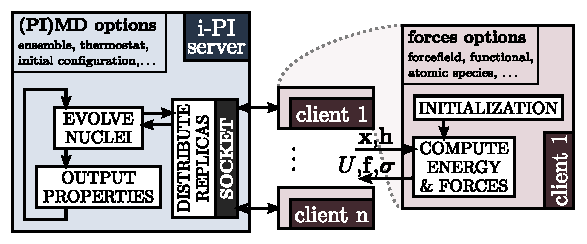
\includegraphics[width=\columnwidth]{ipi-scheme}

  \begin{columns}
    \column{0.5\textwidth}
    \begin{block}{Goal}
      Decouple the problem of evolving the ionic positions and the
      problem of computing the inter-atomic forces.
    \end{block}
    \column{0.5\textwidth}
    \begin{itemize}
      \item i-PI and force calculator on different machine
      \item Crash-safe mechanism
      \item Faster than a ``script'' interface
      \item Easy to parallelize with many replicas
    \end{itemize}
  \end{columns}
\end{frame}

\section{i-PI input}

\begin{frame}{A look at the i-PI input}
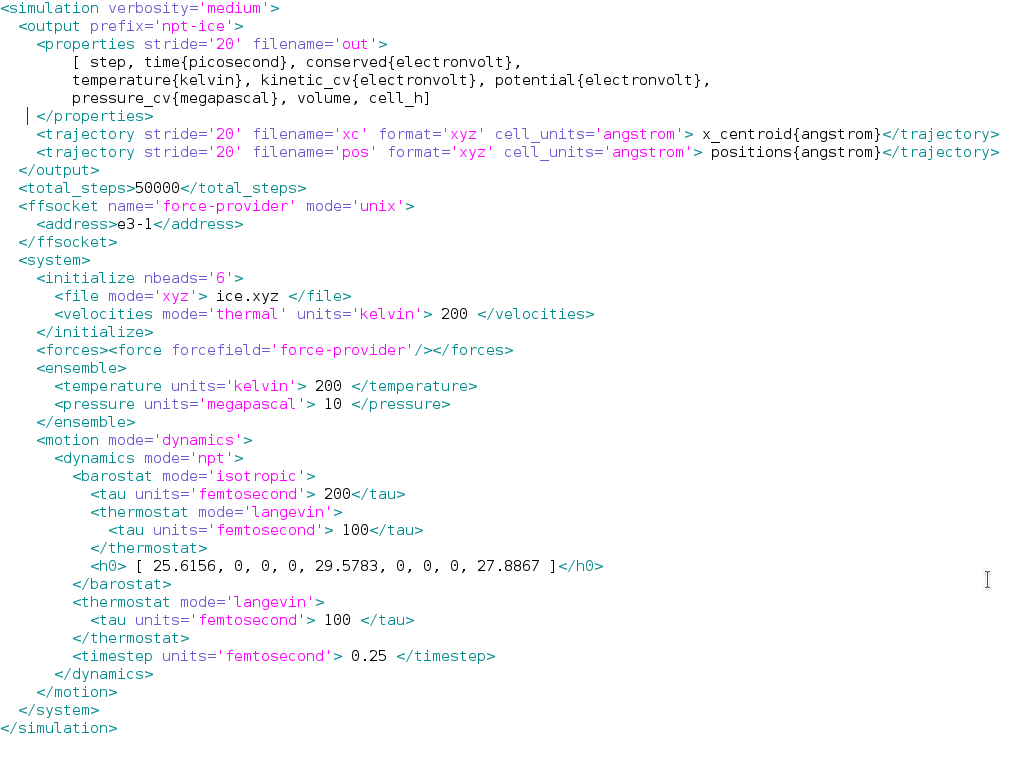
\includegraphics[width=\textwidth]{input_big}
\end{frame}

\begin{frame}{A look at the i-PI input}
\begin{block}{\small XYZ header}
\vspace{1em}
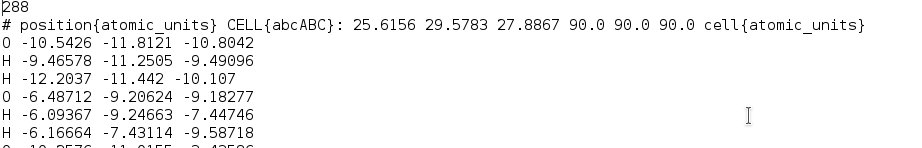
\includegraphics[width=\textwidth]{xyz_header}
\end{block}
\vspace{2.5em}
\begin{block}{\small PDB header}
\vspace{1em}
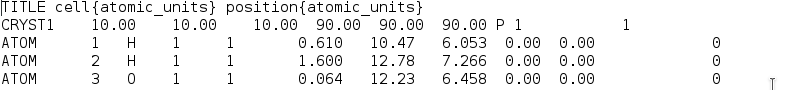
\includegraphics[width=\textwidth]{pdb_header}
\end{block}
\end{frame}

\begin{frame}
Let's start the tutorial\ldots \\
\vspace{2em}
\ldots remember
I am here to answer your questions\ldots
\end{frame}

% \begin{frame}{The Ultimate Goal}
%   \begin{columns}
%     \column{0.5\textwidth}
%     \begin{block}{\small Goals}
%       \small
%       \begin{itemize}
%       \item Reliable and fast approach tuned for organic
%         electronics
%       \item Supramolecular structure description
%       \item Description of challenging systems
%       \end{itemize}
%     \end{block}
%     \vspace{-.4cm}
%     \begin{block}{\small Tools}
%       \small
%       \begin{itemize}
%       \item Dispersion Correction: dDMC\setcounter{footnote}{0}\footnotemark
%       \item REMD@DFTB3\setcounter{footnote}{1}\footnotemark \& REMD@DFTB3-evo\setcounter{footnote}{2}\footnotemark
%       \item New DFA: $\omega$B97X-dDsC\setcounter{footnote}{3}\footnotemark
%       \end{itemize}
%     \end{block}
%     \column{0.5\textwidth}
%     \includegraphics[width=\columnwidth]{intro/nano_solved}
%   \end{columns}
%   \setcounter{footnote}{1}\footnotetext{Petraglia, R.; Steinmann, S.;
%     Corminboeuf, C.\hspace{.5em} \emph{Int. J. Quant. Chem.}
%     \textbf{2015}, \emph{115}, 1265}
%   \setcounter{footnote}{2}\footnotetext{Petraglia, R. \emph{et al.}
%     \hspace{.5em}\emph{J. Comput. Chem.} \textbf{2016}, \emph{37}, 83}
%   \setcounter{footnote}{3}\footnotetext{\textcolor{gray}{Petraglia,
%       R.; Ceriotti, M.; Corminboeuf, C.\hspace{.5em} \emph{In Preparation}}}
%   \setcounter{footnote}{4}\footnotetext{\textcolor{gray}{Fabrizio, A.;
%       Petraglia, R.; Corminboeuf, C.\hspace{.5em} \emph{In Preparation}}}

% \end{frame}

% \note
% {

% \scriptsize Description of the picture.

% We want to develop a QM/MM approach able to describe this kind of
% systems. DFT-MD is computationally too expensive while MM is not able
% to describe the charge mobility: Actually this property make these
% systems so interesting since supramolecular complexes like this can be
% used in organic electronic frameworks.

% We want to go further a merely description of this systems: we want
% understand which are the geometrical key factors (like distance,
% relative orientation, horizontal displacement)
% between $\pi$-delocalized structures, that can improve the charge
% mobility throughout the $pi$-stacked moieties.

% Since DFT cannot be use in large systems, we will use DFTB: that is a
% DFT approximation,  to generate Molecular Dynamics trajectories for
% the big system. Akin to DFT, DFTB suffer for lack of dispersion
% interaction that are really important if we want to study
% $\pi$-stacked systems. The first goal is develop a dispersion correction
% straightforwardly applicable to DFTB scheme. After that we will
% \textcolor{red}{the Verb is missing} the Block-localized wavefunction
% scheme to DFTB in order to be able to use the Marcus-hush theory in
% computing charge mobility.

% To have a finer description of the electronic structure of our system,
% we will provide DFT calculation. Nowadays DFT suffers from two
% challenging shortcoming: charge delocalization error and missing of
% dispersion interactions. To minimize CDE and provide a correction for
% dispersion interaction, we will \textcolor{red}{some verb} a new
% functional based on the existing wB97 and the dDsC dispersion
% correction recently developed at LCMD.

% We assume that reaching this three major achievement will allow the
% description of supramolecular systems organic electronics related and
% the study of those factors able to control the charge mobility in the
% systems.
% }
